\chapter{Results and Conclusion}
\label{ch:results}

This chapter reports every result we obtained. Sections~\ref{sec:res-repro} to~\ref{sec:res-stab} cover the reproduction (the mid-evaluation runs, 50 rounds, one run each), and Sections~\ref{sec:res-nov} and~\ref{sec:res-gate} the extension (20 rounds, two seeds, validation-slice teacher). As explained in Section~\ref{sec:protocols}, numbers from the two protocols are not comparable. All tables and figures are generated from the logs by \texttt{analysis/report\_assets.py} and \texttt{analysis/report\_tables.py}.

\section{Reproduction: comparison with the paper}
\label{sec:res-repro}

Table~\ref{tab:repro} compares our best-round accuracies with the paper's Table~1 (practical setting). Both baselines land close to the published values: FedProto is 0.23 pt below on CIFAR-10, LG-FedAvg 0.28 and 0.51 pt below. The exception is FedProto on CIFAR-100, which is 4.13 pt above the paper. We do not know the exact cause; candidates are HtFLlib's default $\lambda = 10$, a different realisation of the random split, and best-round reporting from a single run. Since the other three baseline numbers agree, we do not think it points to a problem in the pipeline.

The faithful Fed-GDBD reaches 85.70\% and 40.70\%, 2.20 and 4.39 pt below the paper. These are its best rounds, round 1 and round 2, after which it degrades (Section~\ref{sec:res-collapse}). With our fix, FedGDBD-S reaches 87.10\% and 43.74\%: the best of the four methods on both datasets, 0.74 and 0.95 pt above LG-FedAvg, and 0.80 and 1.35 pt below the paper's Fed-GDBD with half the rounds and one run. We beat our own literal implementation, not the paper's reported numbers.

\begin{table}[htbp]
\centering
\caption[Reproduction: our results vs the paper]{Best-round averaged test accuracy (\%) of our runs and the paper's, practical setting ($\beta=0.1$), 20 clients, 50 rounds, one run. $\Delta$ = ours $-$ paper. For FedGDBD-S the paper column repeats the paper's Fed-GDBD. $^\dagger$ best round before the collapse (round 1 and round 2).}
\label{tab:repro}
\small
\TabReproMain
\end{table}

Table~\ref{tab:runs} gives more detail on each run: the round at which the best accuracy occurred, the last-round accuracy, the spread of accuracy across the 20 clients at the best round, and the time per round. For the three stable methods, last and best differ by at most 0.49 pt. The spread across clients is large for every method (about 13 pt on CIFAR-10 and 6 to 9 pt on CIFAR-100), because some clients hold easier classes than others under the skewed split. FedGDBD-S takes about 10 minutes per round against 5 to 10 for the baselines, because each round has two local training phases and a clustering step.

\begin{table}[htbp]
\centering
\caption[Reproduction: details of each run]{Details of each reproduction run. Rounds = training rounds completed; Client SD = standard deviation of the 20 clients' accuracies at the best round (pt); Min/rd. = average minutes per round with three runs sharing one GPU.}
\label{tab:runs}
\scriptsize
\setlength{\tabcolsep}{4pt}
\TabReproRuns
\end{table}

Figure~\ref{fig:convergence} plots the accuracy of all four methods over the 50 rounds. Both Fed-GDBD variants start high, because they begin from pre-trained local models, and are within 1 pt of their best by round 2 to 5, while the baselines need 13 to 31 rounds. We do not count this as a pure advantage of the method, since the baselines start from untrained models. The faithful Fed-GDBD (purple) is the best method for the first rounds and then falls steadily to 75.47\% and 28.00\%; FedGDBD-S (gold) keeps the early lead and stays flat.

\begin{figure}[htbp]
\centering
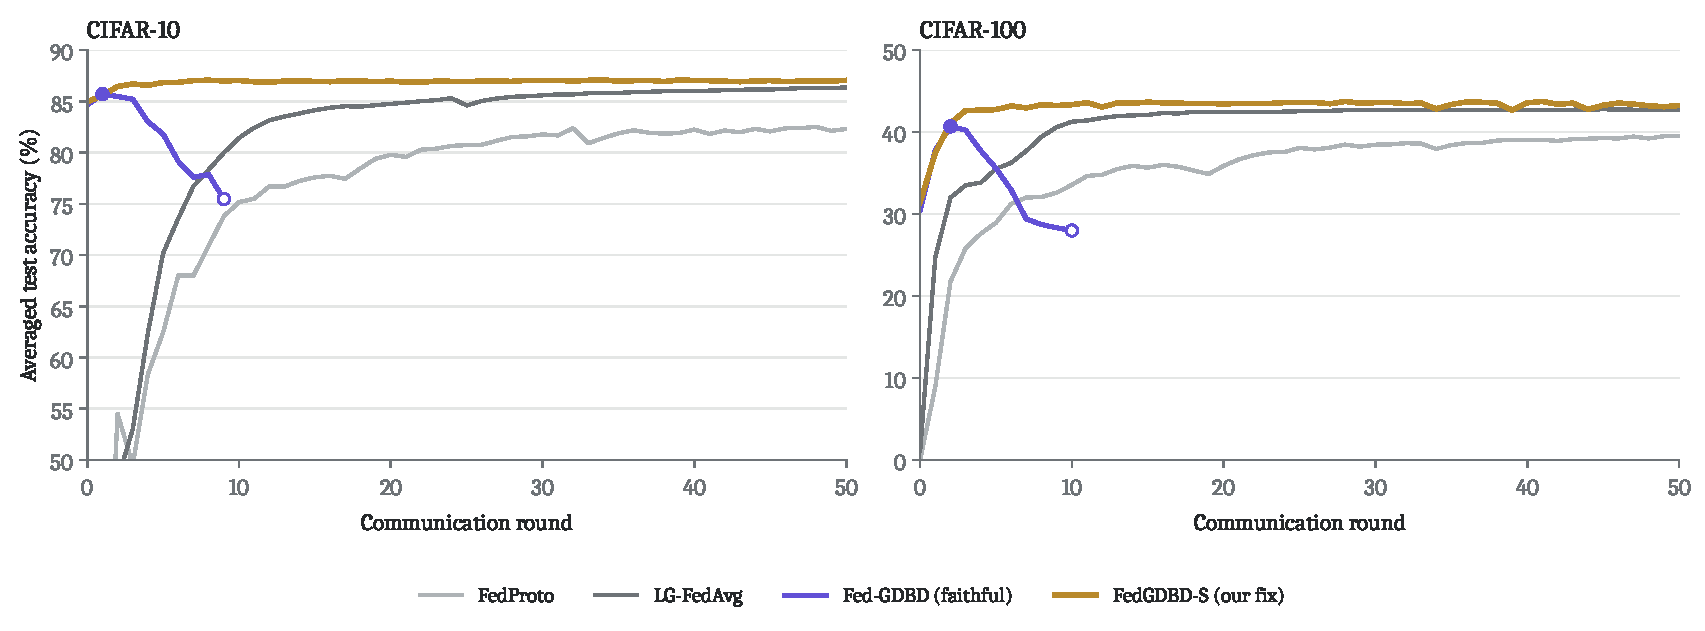
\includegraphics[width=\textwidth]{figures/convergence.pdf}
\caption[Reproduction: accuracy over 50 rounds]{Averaged test accuracy over 50 rounds on CIFAR-10 (left) and CIFAR-100 (right). On the faithful Fed-GDBD line the filled dot marks its best round and the open dot the round at which we stopped it.}
\label{fig:convergence}
\end{figure}

\section{Reproduction: the collapse of the literal update}
\label{sec:res-collapse}

Breaking the accuracy down by architecture shows where the faithful update fails. Table~\ref{tab:collapse} lists the mean accuracy of the five clients of each architecture at the faithful run's best round, at its last round, and for FedGDBD-S at round 50; Figure~\ref{fig:collapse} plots the same numbers.

On CIFAR-100 (Figure~\ref{fig:collapse}b), the CNN clients fall from 48.0\% at round 2 to 3.9\% at round 10, and the ResNet18 clients from 35.7\% to 25.4\%, while GoogLeNet and MobileNetV2 clients keep improving (43.6 to 46.9\% and 35.3 to 36.5\%). On CIFAR-10 (Figure~\ref{fig:collapse}a) the ResNet18 clients suffer most, from 78.7\% to 53.3\%; CNN and GoogLeNet clients lose about 8 pt each and MobileNetV2 clients gain 2.3 pt. The damage is therefore uneven across architectures and different on the two datasets, which is what led us to suspect a mismatch between $g$ and particular feature spaces (Section~\ref{sec:m-fix}). With the fix, every architecture ends at or above the faithful run's best: CIFAR-100 CNN clients recover to 45.6\% and CIFAR-10 ResNet18 clients to 79.2\%.

\begin{table}[htbp]
\centering
\caption[Accuracy per architecture before and after the collapse]{Mean test accuracy (\%) of the five clients of each architecture: faithful Fed-GDBD at its best and last rounds, and FedGDBD-S at round 50.}
\label{tab:collapse}
\small
\TabCollapse
\end{table}

\begin{figure}[htbp]
\centering
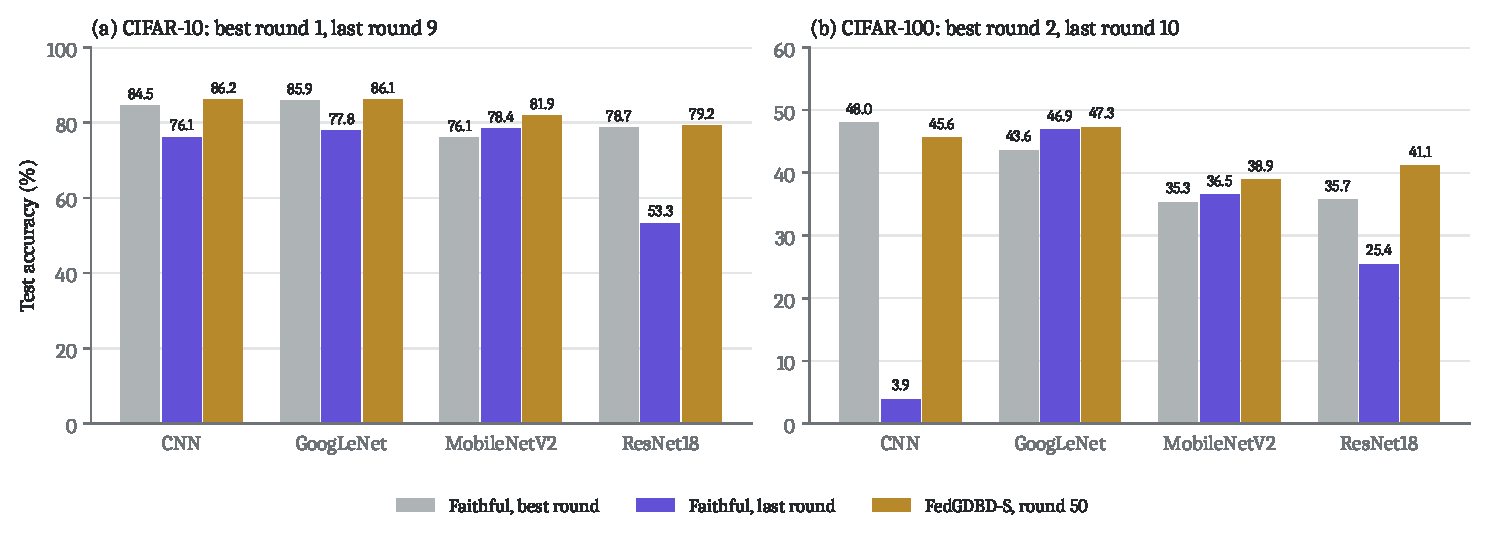
\includegraphics[width=\textwidth]{figures/collapse_both.pdf}
\caption[Collapse of the literal update per architecture]{Accuracy per client architecture for the faithful Fed-GDBD at its best and last rounds, and for FedGDBD-S at round 50. (a) CIFAR-10: the ResNet18 clients fall from 78.7\% to 53.3\% and reach 79.2\% with FedGDBD-S. (b) CIFAR-100: the CNN clients collapse from 48.0\% to 3.9\% and recover to 45.6\%.}
\label{fig:collapse}
\end{figure}

Figure~\ref{fig:ikdbug} answers a natural question: was the collapse caused by our earlier IKD bug (Section~\ref{sec:i-bug})? It was not. The buggy run on CIFAR-100 (grey) peaks at round 2 (41.36\%), declines, and crashes with a NaN loss at round 8. After the fix (purple) the loss stays finite, but the accuracy follows almost the same decline. The bug added a crash; the decline comes from the update in Eq.~\eqref{eq:update}. On CIFAR-10 the buggy run had not diverged when we stopped it after 7 rounds (best 86.82\%, last 84.69\%).

\begin{figure}[htbp]
\centering
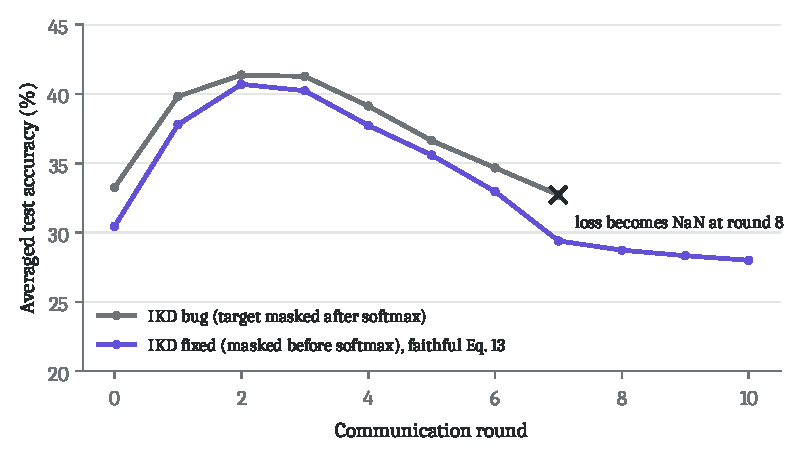
\includegraphics[width=0.72\textwidth]{figures/ikd_bug.pdf}
\caption[Buggy vs fixed IKD loss, CIFAR-100]{CIFAR-100, faithful Fed-GDBD with our first, buggy IKD loss and with the fixed loss. Both decline after round 2; only the buggy one crashes.}
\label{fig:ikdbug}
\end{figure}

\section{Reproduction: per-architecture accuracy of all methods}
\label{sec:res-arch}

Table~\ref{tab:archmethods} and Figure~\ref{fig:archmethods} compare all four methods per architecture at their best rounds. The methods favour different architectures. FedProto is the strongest method on the CNN clients (87.1\% on CIFAR-10, 51.4\% on CIFAR-100) but the weakest on MobileNetV2 (68.6\% and 29.7\%), which suggests that pulling features toward one global mean per class suits some feature extractors far better than others. LG-FedAvg is best on the CIFAR-100 ResNet18 clients (44.3\%). FedGDBD-S is the best on MobileNetV2 on both datasets (81.6\% and 38.8\%) and on GoogLeNet on CIFAR-100 (47.3\%). MobileNetV2 is the hardest architecture for every method.

\begin{table}[htbp]
\centering
\caption[Per-architecture accuracy of all methods]{Mean test accuracy (\%) per client architecture for each method at its best round.}
\label{tab:archmethods}
\small
\TabArchMethods
\end{table}

\begin{figure}[htbp]
\centering
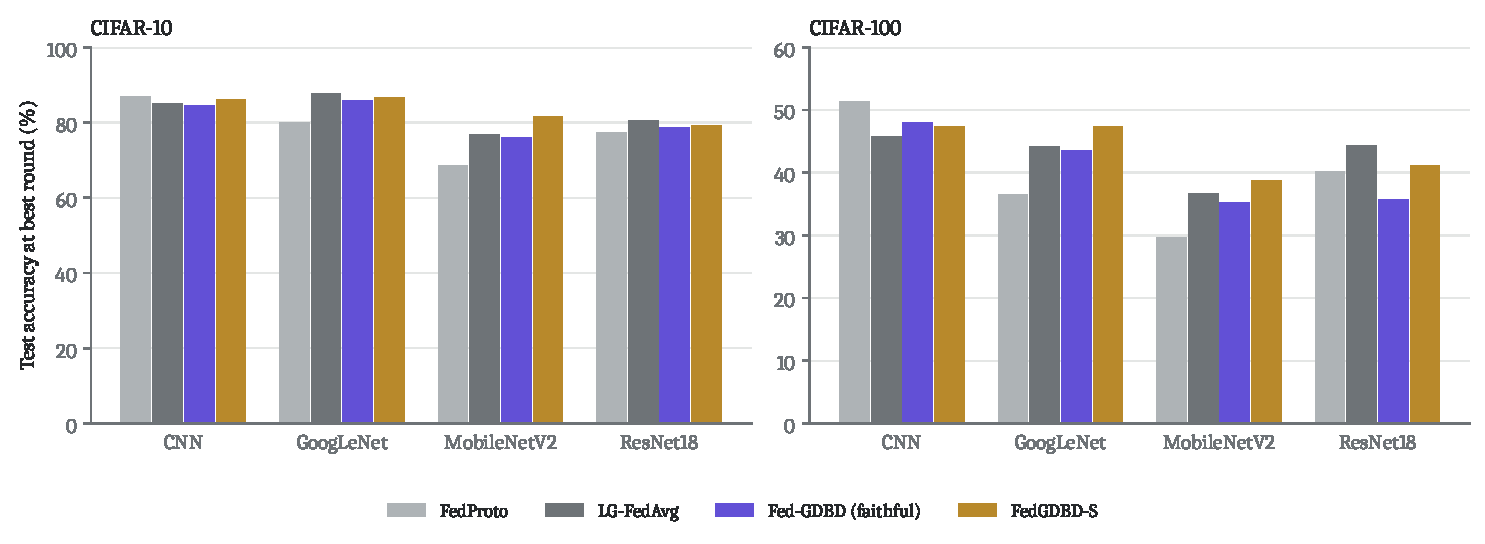
\includegraphics[width=\textwidth]{figures/per_arch_methods.pdf}
\caption[Per-architecture accuracy of all methods]{Accuracy per client architecture for the four methods at their best rounds, CIFAR-10 (left) and CIFAR-100 (right).}
\label{fig:archmethods}
\end{figure}

\section{Reproduction: stability of FedGDBD-S}
\label{sec:res-stab}

FedGDBD-S shows no downward trend over 50 rounds (Figure~\ref{fig:convergence}). From round 3 onward its accuracy never drops more than 0.53 pt below its best on CIFAR-10 and 1.1 pt on CIFAR-100; the larger dips on CIFAR-100 are single rounds (for example 42.70\% at round 39) followed by recovery. Its best rounds were 34 and 28, and its last-round accuracies 87.06\% and 43.25\%.

\section{Extension: agreement-gated distillation}
\label{sec:res-nov}

Table~\ref{tab:novbest} gives the best-round accuracy of the control (FedGDBD-S) and of the two gates for both seeds, with two-seed means and the gap to the control. Figure~\ref{fig:novconv} shows the accuracy curves of all twelve runs.

\begin{table}[htbp]
\centering
\caption[Extension: best-round accuracy]{Extension runs: best-round averaged test accuracy (\%), 20 rounds, validation-slice teacher. The gap is the difference of two-seed means to the control.}
\label{tab:novbest}
\small
\TabNovBest
\end{table}

The per-seed gaps to the control are:
\begin{itemize}
\item AGC on CIFAR-100: $+0.86$ and $+0.52$ (mean $+0.69$).
\item AGS on CIFAR-10: $+0.40$ and $+0.37$ (mean $+0.39$).
\item AGC on CIFAR-10: $-0.04$ and $+0.45$ (mean $+0.21$).
\item AGS on CIFAR-100: $+0.17$ and $-0.14$ (mean $+0.02$).
\end{itemize}
Measured against the criterion fixed before the runs (at least $+0.5$ pt on both datasets), neither gate is an improvement, and we do not claim a general gain. Two results do repeat across both seeds: AGC helps on CIFAR-100 and AGS helps on CIFAR-10. In both cases the gain in each seed is larger than the control's own change between seeds (0.19 and 0.23 pt). With two seeds this is evidence, not proof.

\begin{figure}[htbp]
\centering
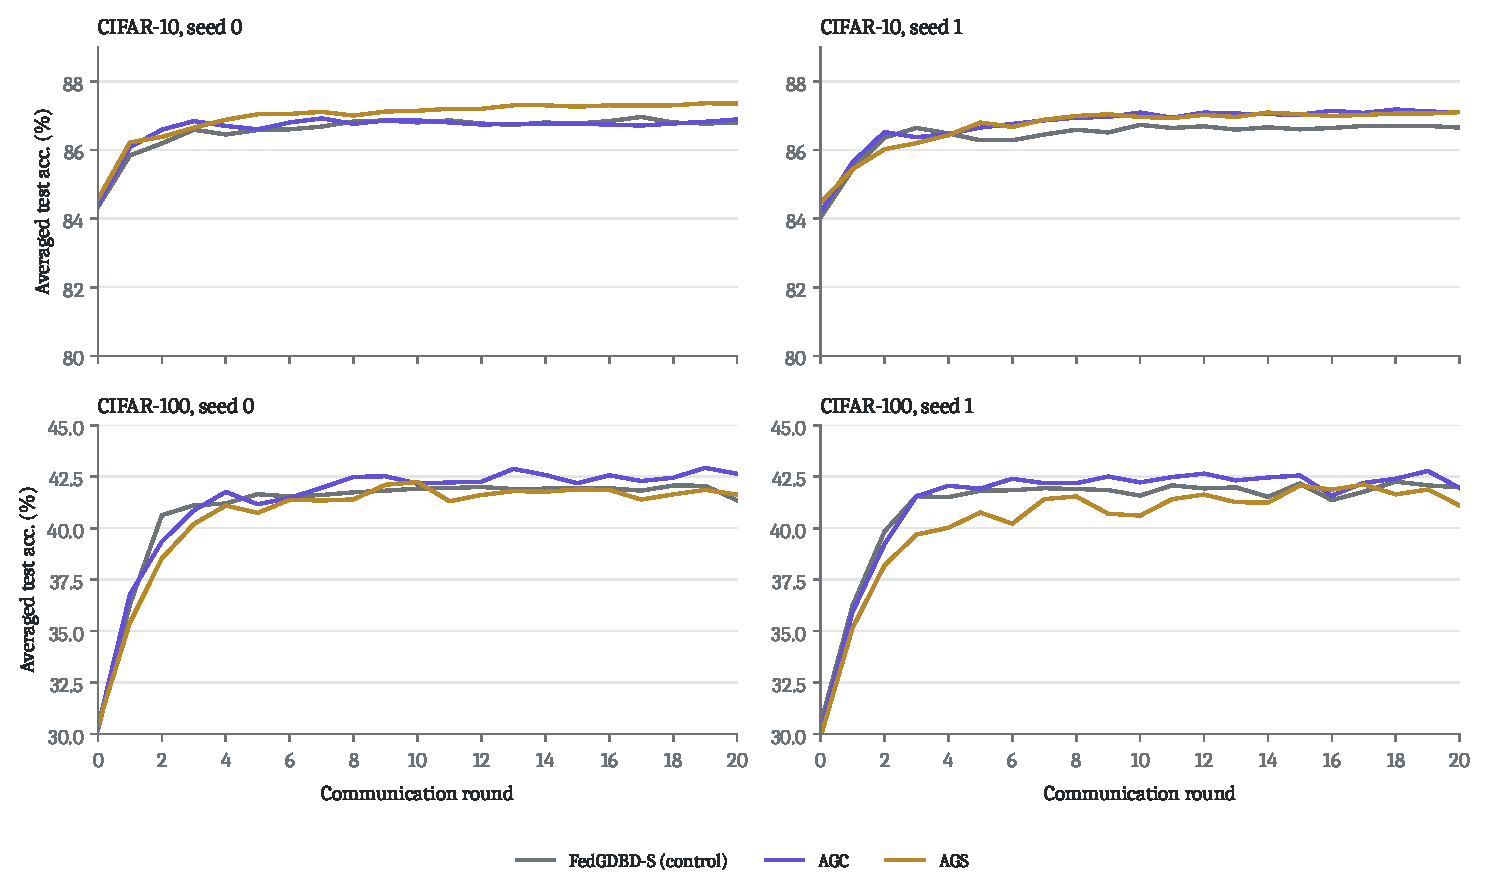
\includegraphics[width=\textwidth]{figures/novelty_convergence.pdf}
\caption[Extension: accuracy over 20 rounds]{Averaged test accuracy over 20 rounds for the control and the two gates, by dataset (rows) and seed (columns).}
\label{fig:novconv}
\end{figure}

The curves in Figure~\ref{fig:novconv} show the same picture over the whole run rather than only at the best round. On CIFAR-10, AGS is above the control in every round of seed 0 and in every round from round 5 of seed 1. On CIFAR-100, AGC is above the control in almost every round after the first few, in both seeds, while AGS stays below it in most rounds: in its first rounds it discards almost all MobileNetV2 images (Section~\ref{sec:res-gate}).

Because best-round reporting is slightly optimistic, Table~\ref{tab:novlast} repeats the comparison at the last round. The conclusions do not change: AGC is $+0.63$ pt above the control on CIFAR-100 and AGS $+0.50$ pt on CIFAR-10, while AGS on CIFAR-100 is now 0.30 pt below.

\begin{table}[htbp]
\centering
\caption[Extension: last-round accuracy]{Extension runs: last-round (round 20) averaged test accuracy (\%).}
\label{tab:novlast}
\small
\TabNovLast
\end{table}

Table~\ref{tab:novarch} lists per-architecture accuracy at the best round for every extension run, and Table~\ref{tab:archgain} with Figure~\ref{fig:archgain} the two-seed mean gain of each gate over the control per architecture. On CIFAR-10 the MobileNetV2 clients gain the most under both gates ($+0.95$ with AGC, $+1.13$ with AGS). On CIFAR-100, AGC helps ResNet18 ($+1.33$) and MobileNetV2 ($+0.87$) most, and AGS costs the CNN clients 0.91 pt, which explains why AGS does not help there overall.

\begin{table}[htbp]
\centering
\caption[Extension: per-architecture accuracy, every run]{Extension runs: mean test accuracy (\%) per client architecture at each run's best round.}
\label{tab:novarch}
\scriptsize
\setlength{\tabcolsep}{4pt}
\TabNovArch
\end{table}

\begin{table}[htbp]
\centering
\caption[Extension: per-architecture gain over the control]{Gain of each gate over the control per architecture (pt), mean of the two seeds, at the best round.}
\label{tab:archgain}
\small
\TabArchGain
\end{table}

\begin{figure}[htbp]
\centering
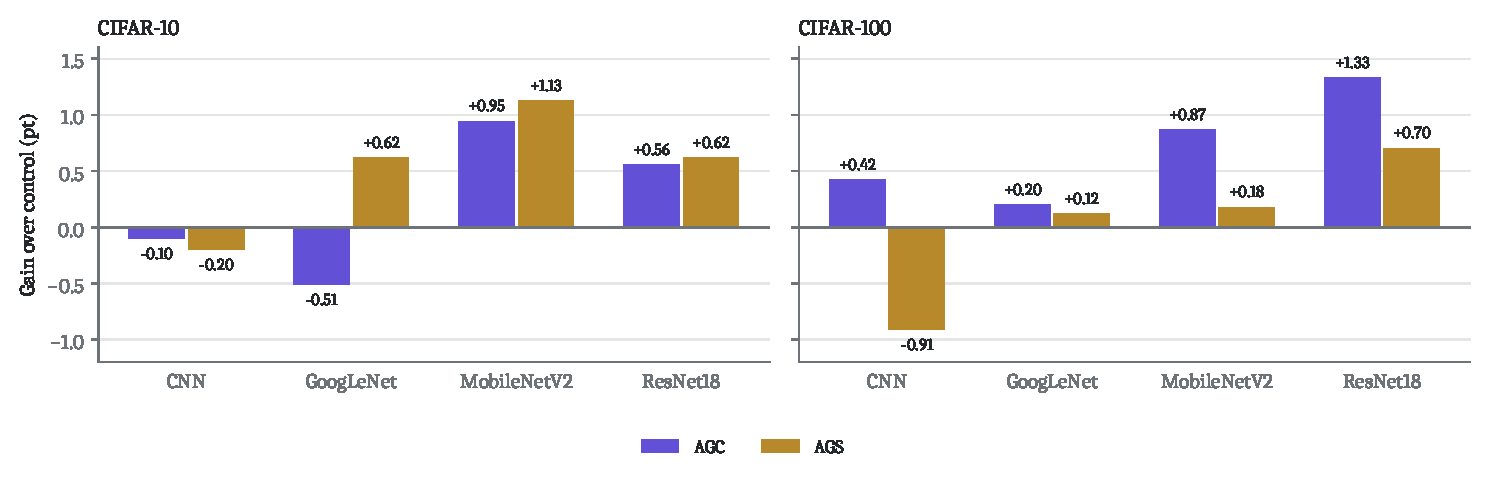
\includegraphics[width=\textwidth]{figures/arch_gains.pdf}
\caption[Extension: per-architecture gain over the control]{Per-architecture gain of AGC and AGS over the control, two-seed means, CIFAR-10 (left) and CIFAR-100 (right).}
\label{fig:archgain}
\end{figure}

\section{Extension: what the gates measured}
\label{sec:res-gate}

The gate statistics in the logs describe how well $g$ fits each architecture. Table~\ref{tab:gate} summarises them, and Figures~\ref{fig:gacc} and~\ref{fig:kept} show how they change over the rounds.

\begin{table}[htbp]
\centering
\caption[Gate statistics per architecture]{Gate statistics per architecture, seed 0 / seed 1. AGC rows: share of the clients' training images that $g$ classifies correctly (the value that scales $\alpha$). AGS rows: share of images actually distilled.}
\label{tab:gate}
\scriptsize
\setlength{\tabcolsep}{4pt}
\TabGate
\end{table}

Measured by AGC, $g$ classifies 96 to 97\% of the CNN clients' CIFAR-10 training images correctly over the run, but only 49 to 53\% of the MobileNetV2 clients'. On CIFAR-100 the figures are 75 to 81\% for CNN, GoogLeNet and ResNet18 against 42 to 44\% for MobileNetV2. At round 0 the gap is extreme: $g$ is right on 11 to 14\% of MobileNetV2 images on CIFAR-10 and 2 to 3\% on CIFAR-100. The gate was never told about architectures, yet in all four runs it singles out MobileNetV2 as the architecture $g$ serves worst.

\begin{figure}[htbp]
\centering
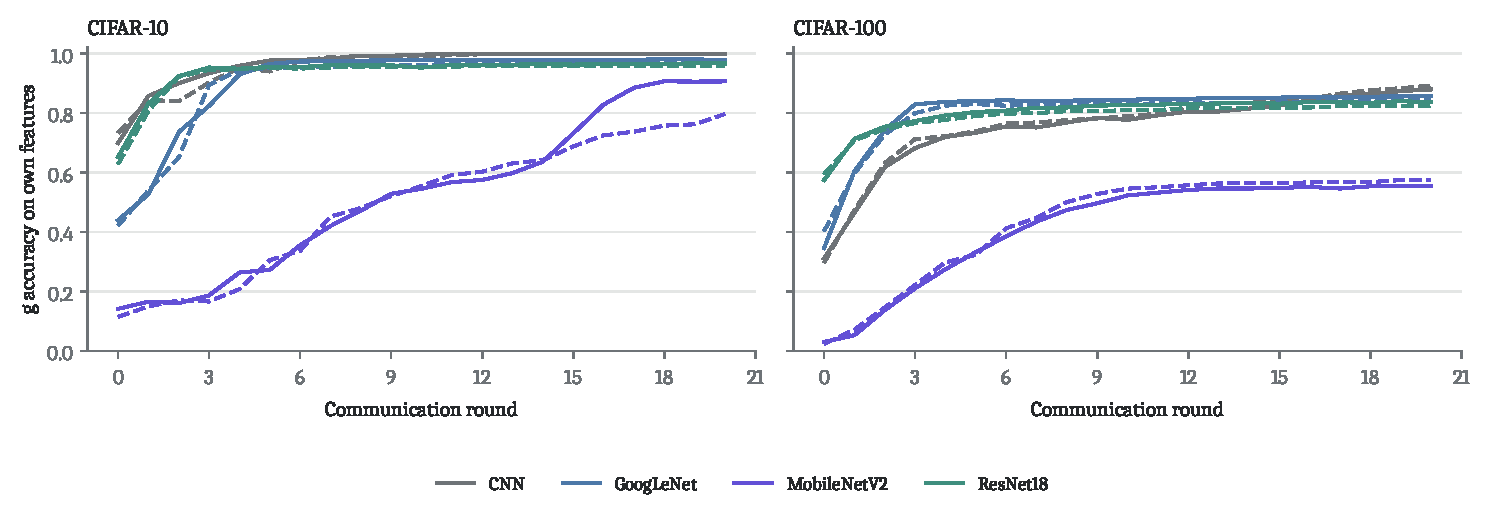
\includegraphics[width=\textwidth]{figures/gate_gacc.pdf}
\caption[AGC: accuracy of $g$ per architecture over rounds]{AGC: accuracy of $g$ on each architecture's own training features over the rounds (solid: seed 0, dashed: seed 1). MobileNetV2 starts far below the others and catches up only partly.}
\label{fig:gacc}
\end{figure}

Figure~\ref{fig:gacc} shows that $g$'s accuracy on MobileNetV2 features rises over the run as $g$ and the clients adapt, to about 0.8 to 0.9 on CIFAR-10 by round 20 and about 0.56 on CIFAR-100, while the other architectures pass 0.7 within about five rounds. So the gate reduces MobileNetV2's distillation weight most in the early rounds and less later.

\begin{figure}[htbp]
\centering
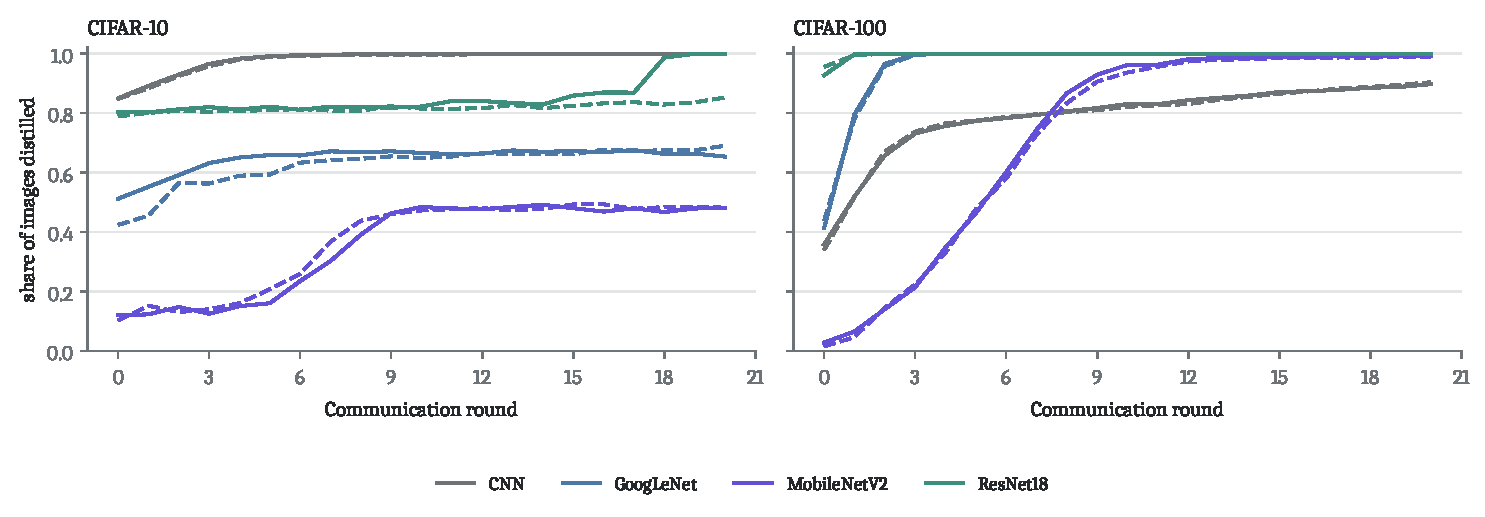
\includegraphics[width=\textwidth]{figures/gate_kept.pdf}
\caption[AGS: share of images distilled over rounds]{AGS: share of each architecture's images that were distilled in each round (solid: seed 0, dashed: seed 1).}
\label{fig:kept}
\end{figure}

AGS (Figure~\ref{fig:kept}) shows the same pattern from a different angle. On CIFAR-10, MobileNetV2 clients distil only 36 to 37\% of their images on average and GoogLeNet clients 62 to 65\%, while CNN clients distil 98\%. On CIFAR-100 nearly all images of the GoogLeNet and ResNet18 clients are distilled after a few rounds, MobileNetV2 climbs from 1 to 3\% at round 0 to almost all, and the CNN clients rise slowly from about 35\% to about 90\%. These kept fractions are counted during training (model in training mode), so they differ from AGC's evaluation-mode accuracy, but both point to MobileNetV2.

\section{Discussion}
\label{sec:discussion}

\textbf{Why the literal update collapses.} The collapse hits different architectures on the two datasets and builds up over several rounds. Both facts fit our explanation: a scale mismatch between $g$'s logits and some clients' heads, amplified by the KD weight $\alpha T^2 = 280$, so that distillation overrides cross-entropy and reshapes the extractor. The fix works by removing exactly these two channels (the scale and the gradient into the extractor), which supports the explanation, but we did not log logit norms to confirm it directly. The authors' unreleased code may include a detail that avoids the problem, such as a normalisation or a smaller learning rate.

\textbf{Why each gate helps a different dataset.} This is our interpretation and not proven. On CIFAR-100, $g$ is wrong often, but its softened predictions still carry information about which of the 100 classes look alike, so turning the distillation down smoothly (AGC) keeps that information while reducing the harm. Discarding images (AGS) throws it away, and in the first rounds AGS discards almost all MobileNetV2 images. On CIFAR-10, $g$ is right on most images and there are only 10 classes, so removing only the images $g$ gets wrong (AGS) cleans up the signal without losing much.

\textbf{The architecture finding.} The clearest result of the extension is not an accuracy gain but a measurement: one linear boundary shared by four architectures fits them very unequally, and the unevenness is large (about 0.5 vs 0.97 on CIFAR-10). It matches what the baselines show in Table~\ref{tab:archmethods}, where MobileNetV2 is the hardest architecture for every method and FedProto, which also imposes one global target per class, is weakest exactly there. The gains follow the measurement on CIFAR-10, where MobileNetV2 benefits most; on CIFAR-100 the largest AGC gain goes to ResNet18, so the link is not one-to-one.

\textbf{Threats to validity.} Two seeds cannot give a reliable estimate of a 0.4 pt effect. All accuracies are best-round values, as in the paper, which is optimistic; the last-round results agree, which reduces this concern. In the reproduction the IKD teacher was picked by test accuracy, a mild use of test data shared by Fed-GDBD and FedGDBD-S; the extension runs avoid it. GPU nondeterminism and the unseeded client order in the reproduction runs mean a rerun will differ slightly.

\section{Limitations}

\begin{table}[htbp]
\centering
\caption[Limitations and remedies]{Limitations of this study and what would address them.}
\label{tab:limits}
\small
\begin{tabularx}{\textwidth}{>{\raggedright\arraybackslash}X>{\raggedright\arraybackslash}p{3.4cm}>{\raggedright\arraybackslash}X}
\toprule
Limitation & Reason & Remedy \\
\midrule
Two of the paper's four datasets; practical split only & compute & Tiny-ImageNet, Flowers102, pathological split \\
Reproduction: 50 rounds, one run (paper: 100 $\times$ 3) & compute & full-length runs with three seeds \\
Extension: two seeds, 20 rounds & compute & five or more seeds, reported as mean $\pm$ SD \\
Collapse explanation not proven & no logit statistics logged & log logit scales per architecture \\
No ablation of $\alpha$, $T$, or a fixed smaller $\alpha$ for all clients & time & run these as additional controls \\
Only FedProto and LG-FedAvg as baselines & compute & add FedTGP and FedGH (already in HtFLlib) \\
\bottomrule
\end{tabularx}
\end{table}

Table~\ref{tab:limits} lists the main limitations. The missing control for AGC deserves a note: AGC lowers the distillation weight only for clients $g$ misreads, and well-served clients keep almost the paper's value, so it is not the same as lowering $\alpha$ for everyone. But we did not run that comparison, and it is the first one a sceptical reader would ask for.

\section{Future work}

\begin{enumerate}
\item Repeat the extension with five or more seeds and report mean $\pm$ standard deviation, so that effects of a few tenths of a point can be measured properly.
\item Run 50 to 100 rounds, the paper's other datasets and the pathological split.
\item Add the missing controls: a sweep over $\alpha$ and $T$ and a run with one smaller $\alpha$ for all clients.
\item Try a soft gate, using $g$'s probability for the true label as the weight instead of a 0/1 decision, and a hybrid that uses AGC where $\mathrm{acc}_i$ is low and AGS where it is high.
\item Test the collapse explanation directly by logging the logit scales of $g$ and of each head per architecture.
\end{enumerate}

\section{Conclusion}

We re-implemented Fed-GDBD from its paper and reproduced its main experiment on CIFAR-10 and CIFAR-100. The baselines matched the published numbers closely, which gives confidence in the setup. The literal client update turned out to be unstable for particular architectures; two changes to the distillation step, logit-scale matching and head-only distillation, fixed it without touching the paper's hyper-parameters, and the fixed version was the best method in our runs, about one point below the paper's reported results with half the training.

Our extension gates the distillation of the global boundary by whether it agrees with each client's labels. It gave gains that repeated across two seeds on one dataset each (AGC on CIFAR-100, AGS on CIFAR-10), but it did not meet the bar we set in advance, and we do not claim that it improves Fed-GDBD in general. Its main lasting result is the measurement behind it: a single global boundary fits some client architectures far worse than others, and a client can detect this from its own data at no communication cost. Measuring that properly, with more seeds and the missing controls, is the natural next step.
